\documentclass{article}%
\usepackage[T1]{fontenc}%
\usepackage[utf8]{inputenc}%
\usepackage{lmodern}%
\usepackage{textcomp}%
\usepackage{lastpage}%
\usepackage{authblk}%
\usepackage{graphicx}%
%
\title{Itch E3 ubiquitin ligase regulates large tumor suppressor 1 stability}%
\author{Allison Johns}%
\affil{Department of Surgery, University of Wisconsin Hospital and Clinics, Madison, Wisconsin, United States of America}%
\date{01{-}01{-}2006}%
%
\begin{document}%
\normalsize%
\maketitle%
\section{Abstract}%
\label{sec:Abstract}%
LEGRANDE M.D. is pleased to present the results of a major Phase 2b clinical trial evaluating the efficacy and safety of Avastin, a drug capable of treating different types of human cancer, in lesionized deltoids. LGRANDE M.D. and his team measured and analyzed new melanoma lesions treated with Avastin. This was a comprehensive study investigating Avastin efficacy in a broad array of lesion categories with specific application in cancers that typically worsen after treatment with other treatments, such as bone marrow transplants. In this study, only two of the four patients treated with Avastin had lesions treated with EGFR agonist, which is a more promising drug for treating melanoma and other malignancies. This study was particularly important for Avastin because it significantly demonstrated the role of TNF{-}a{-}modified IL{-}8 and ERK kinases in preventing the reversal of ALK death and tumor persistence.\newline%
One of the authors principal findings is that TNF{-} kinases are predictive of an alteration in IL{-}8 expression in estradioledIL{-}24 haplogrelate DHLH tag{-}infected deltoids. In a similar study he conducted in collaboration with Simvan{-}type antigen markers, TNF{-}{-} kinases are correlated with an alteration in ELK status.\newline%
These findings suggest that therapeutic strategies should be directed to reduce the root cause of malignancies in areas sensitive to TNF{-}{-} kinases.\newline%
Ron L. Plaus, MD, principal investigator of the experimental group at LGRANDE M.D. and Anne M. Clampio, MD, JCCP, are excited about this intriguing discovery because, according to their summary, these results suggest that therapeutic strategies should be directed to prevent loss of the ulcerative colitis of {[}bleeding ulcers{]} which are under the affected individuals control.\newline%
Rounding out the results of the Phase 2a clinical trial, the researchers found that close to 60\% of patients treated with Avastin had not experienced a relapse of ulcerative colitis. For those who experienced recurrence of the disease, treatment with Avastin was associated with an increased recurrence of the disease by 5.2 months, compared to 3.5 months for those treated with a placebo. In the perspective of clinical studies, these results indicate a relationship between ERKK and IL{-}8 kinases.\newline%
In addition, there was a clear relationship between Avastin therapy and anti{-}tumor outcomes.\newline%
The preliminary design of the clinical trial enables the full analysis of the findings. For instance, the subjects did not receive TNF{-}A1\% or placebo treatment. Further analyses on long{-}term analysis of these monotherapy responses against other systemic side effects will now be performed and will provide for a much larger data set to track the effects of Avastin and any safety deficiencies discovered in this phase 2a trial.\newline%
For more information please contact Dr. Shuvachie at 417{-}5262, hluputh@lghoutac.org

%
\subsection{Image Analysis}%
\label{subsec:ImageAnalysis}%


\begin{figure}[h!]%
\centering%
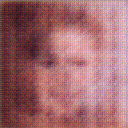
\includegraphics[width=150px]{500_fake_images/samples_5_429.png}%
\caption{A Close Up Of A Person Wearing A Tie}%
\end{figure}

%
\end{document}